Das von uns entwickelte Programm zur Untersuchung des Ising-Modells ist in C geschrieben. Die wichtigen Parameter zum steuern der Simulation werden als Programmparameter beim starten mitgegeben. Die Zufallszahlen im Programm werden mit einem Mersenne-Twister Pseudozufallszahlengenerator erzeugt.

\subsection{Metropolis Schema}

1. Es ist ein Anfangszustand gegeben\\
2. Wähle zufällig einen Spin aus\\
3. Berechne die Energiedifferenz $\Delta E$ gegenüber dem jetzigen Zustand, wenn der gewählte Spin geflippt wird\\
4. Flippe den Spin mit Wahrscheinlichkeit $P(S_k \rightarrow -S_k)=min\{ 1, e^{(-\frac{\Delta E}{k_B T})} \}$\\
5. Gehe zu 1.\\\\
In unserem Programm bilden $N^{dim}$ Durchläufe dieses Schemas einen Monte-Carlo-Schritt (step).

\subsection{Im Detail: Konvergenz des Metropolis Algorithmus}

Hier der Metropolis Block eines Monte Carlo Schritts mit Konvergenzverhalten

2D

\begin{figure}[H]
	\centering
	\subfigure[zufällige Startkonfiguration]{
		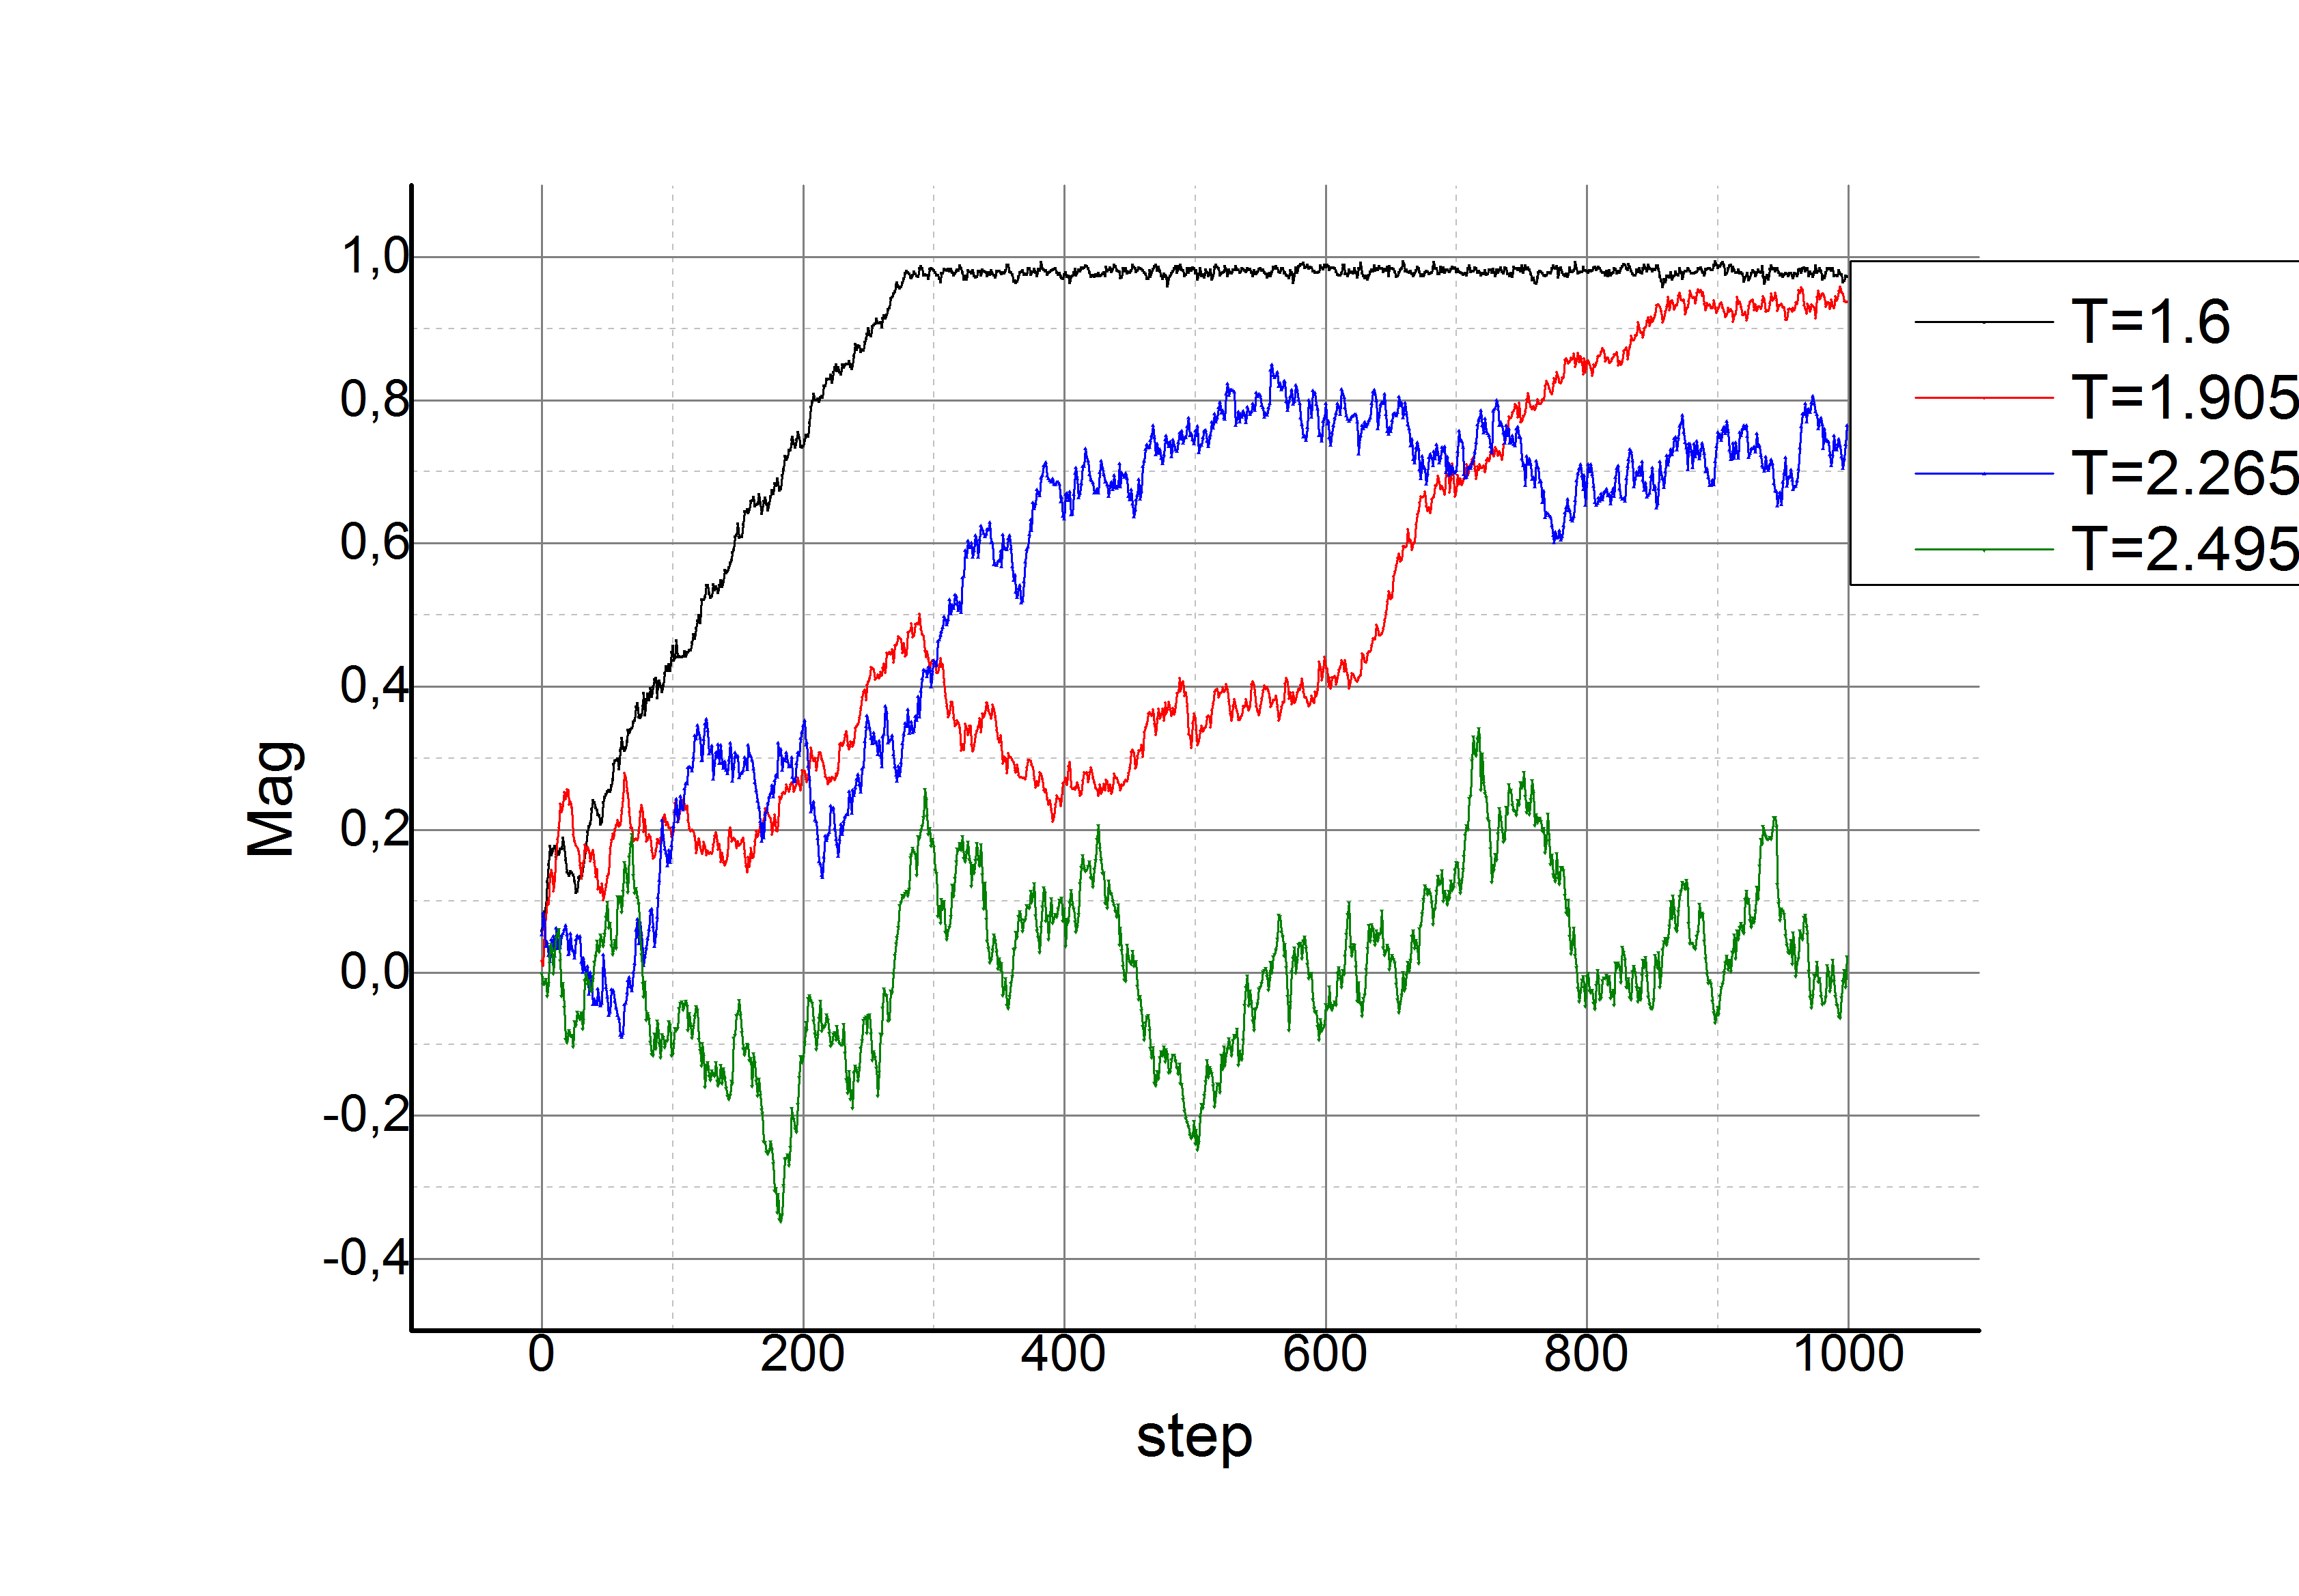
\includegraphics[width=0.47\textwidth]{../Graph_Export/MP2D/m(Steps)_r.jpg}
}	
	\subfigure[positv parallele Startkonfiguration]{
		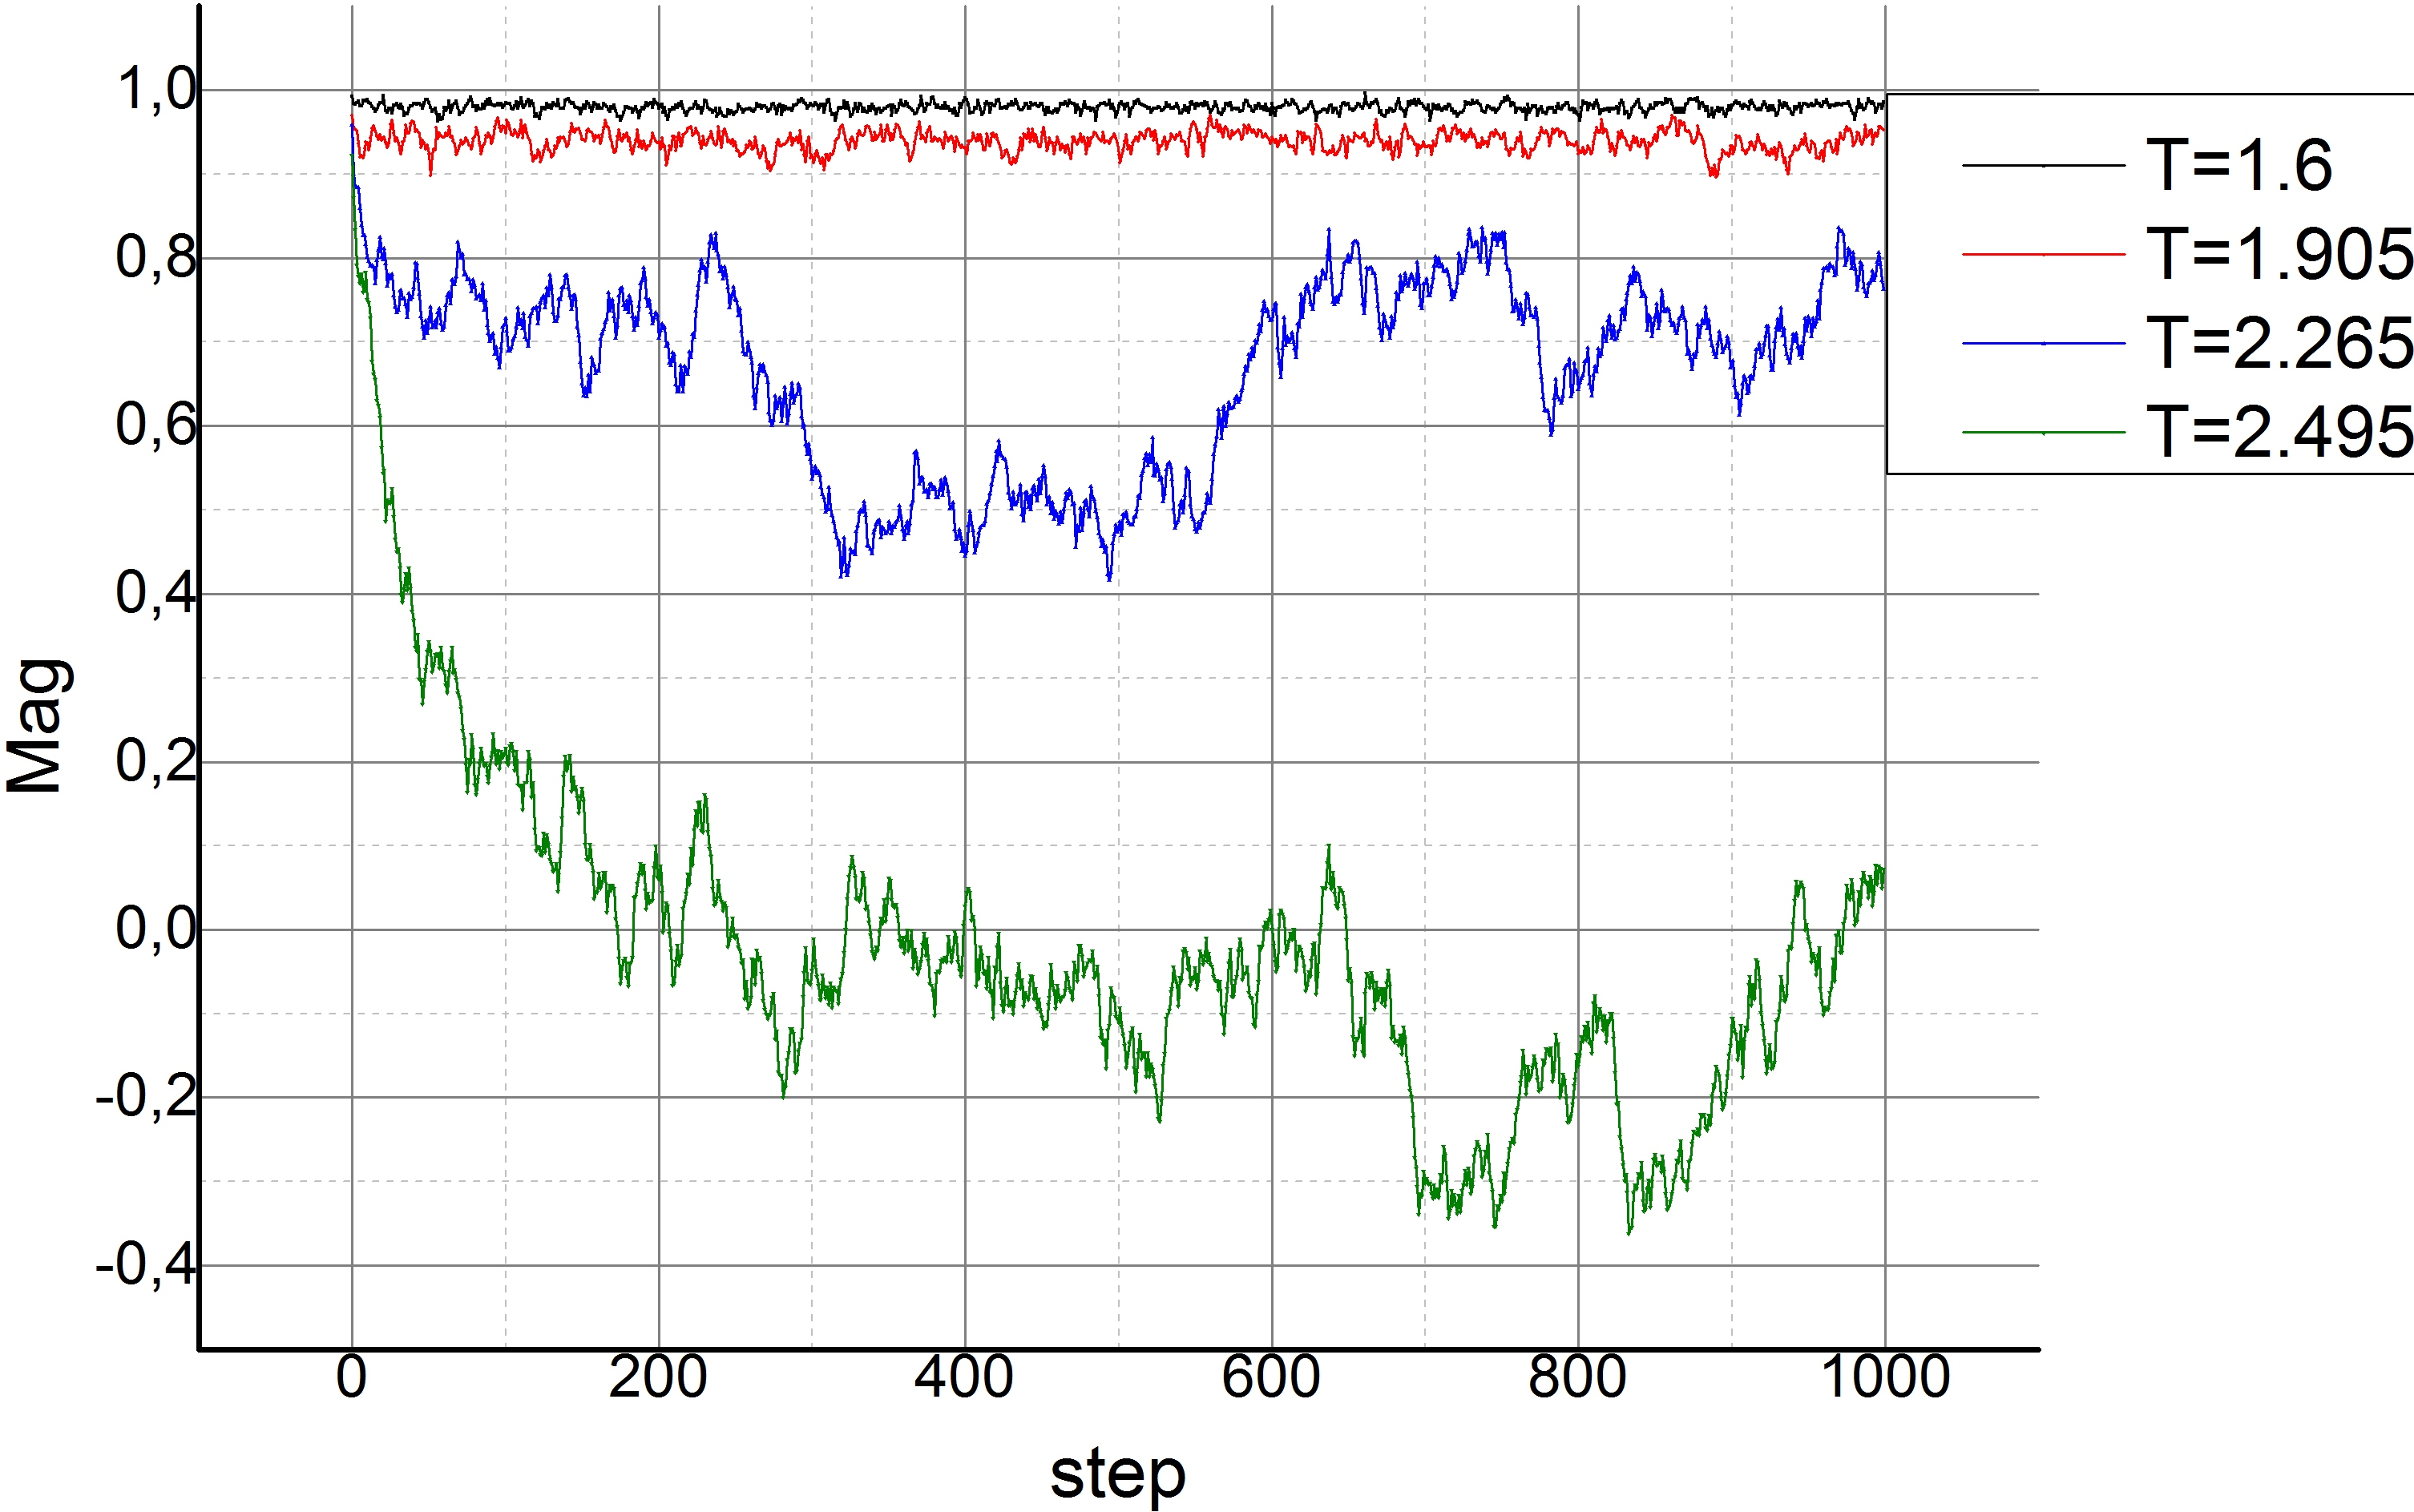
\includegraphics[width=0.47\textwidth]{../Graph_Export/MP2D/m(Steps)_p.jpg}
}		
	\caption{Konvergenzverhalten der Magnetisierung im Metropolisalgorithmus für ein zweidimensionales Gitter}
	\label{mp2dkonv}
\end{figure}

3D

\begin{figure}[H]
	\centering
	\subfigure[zufällige Startkonfiguration]{
		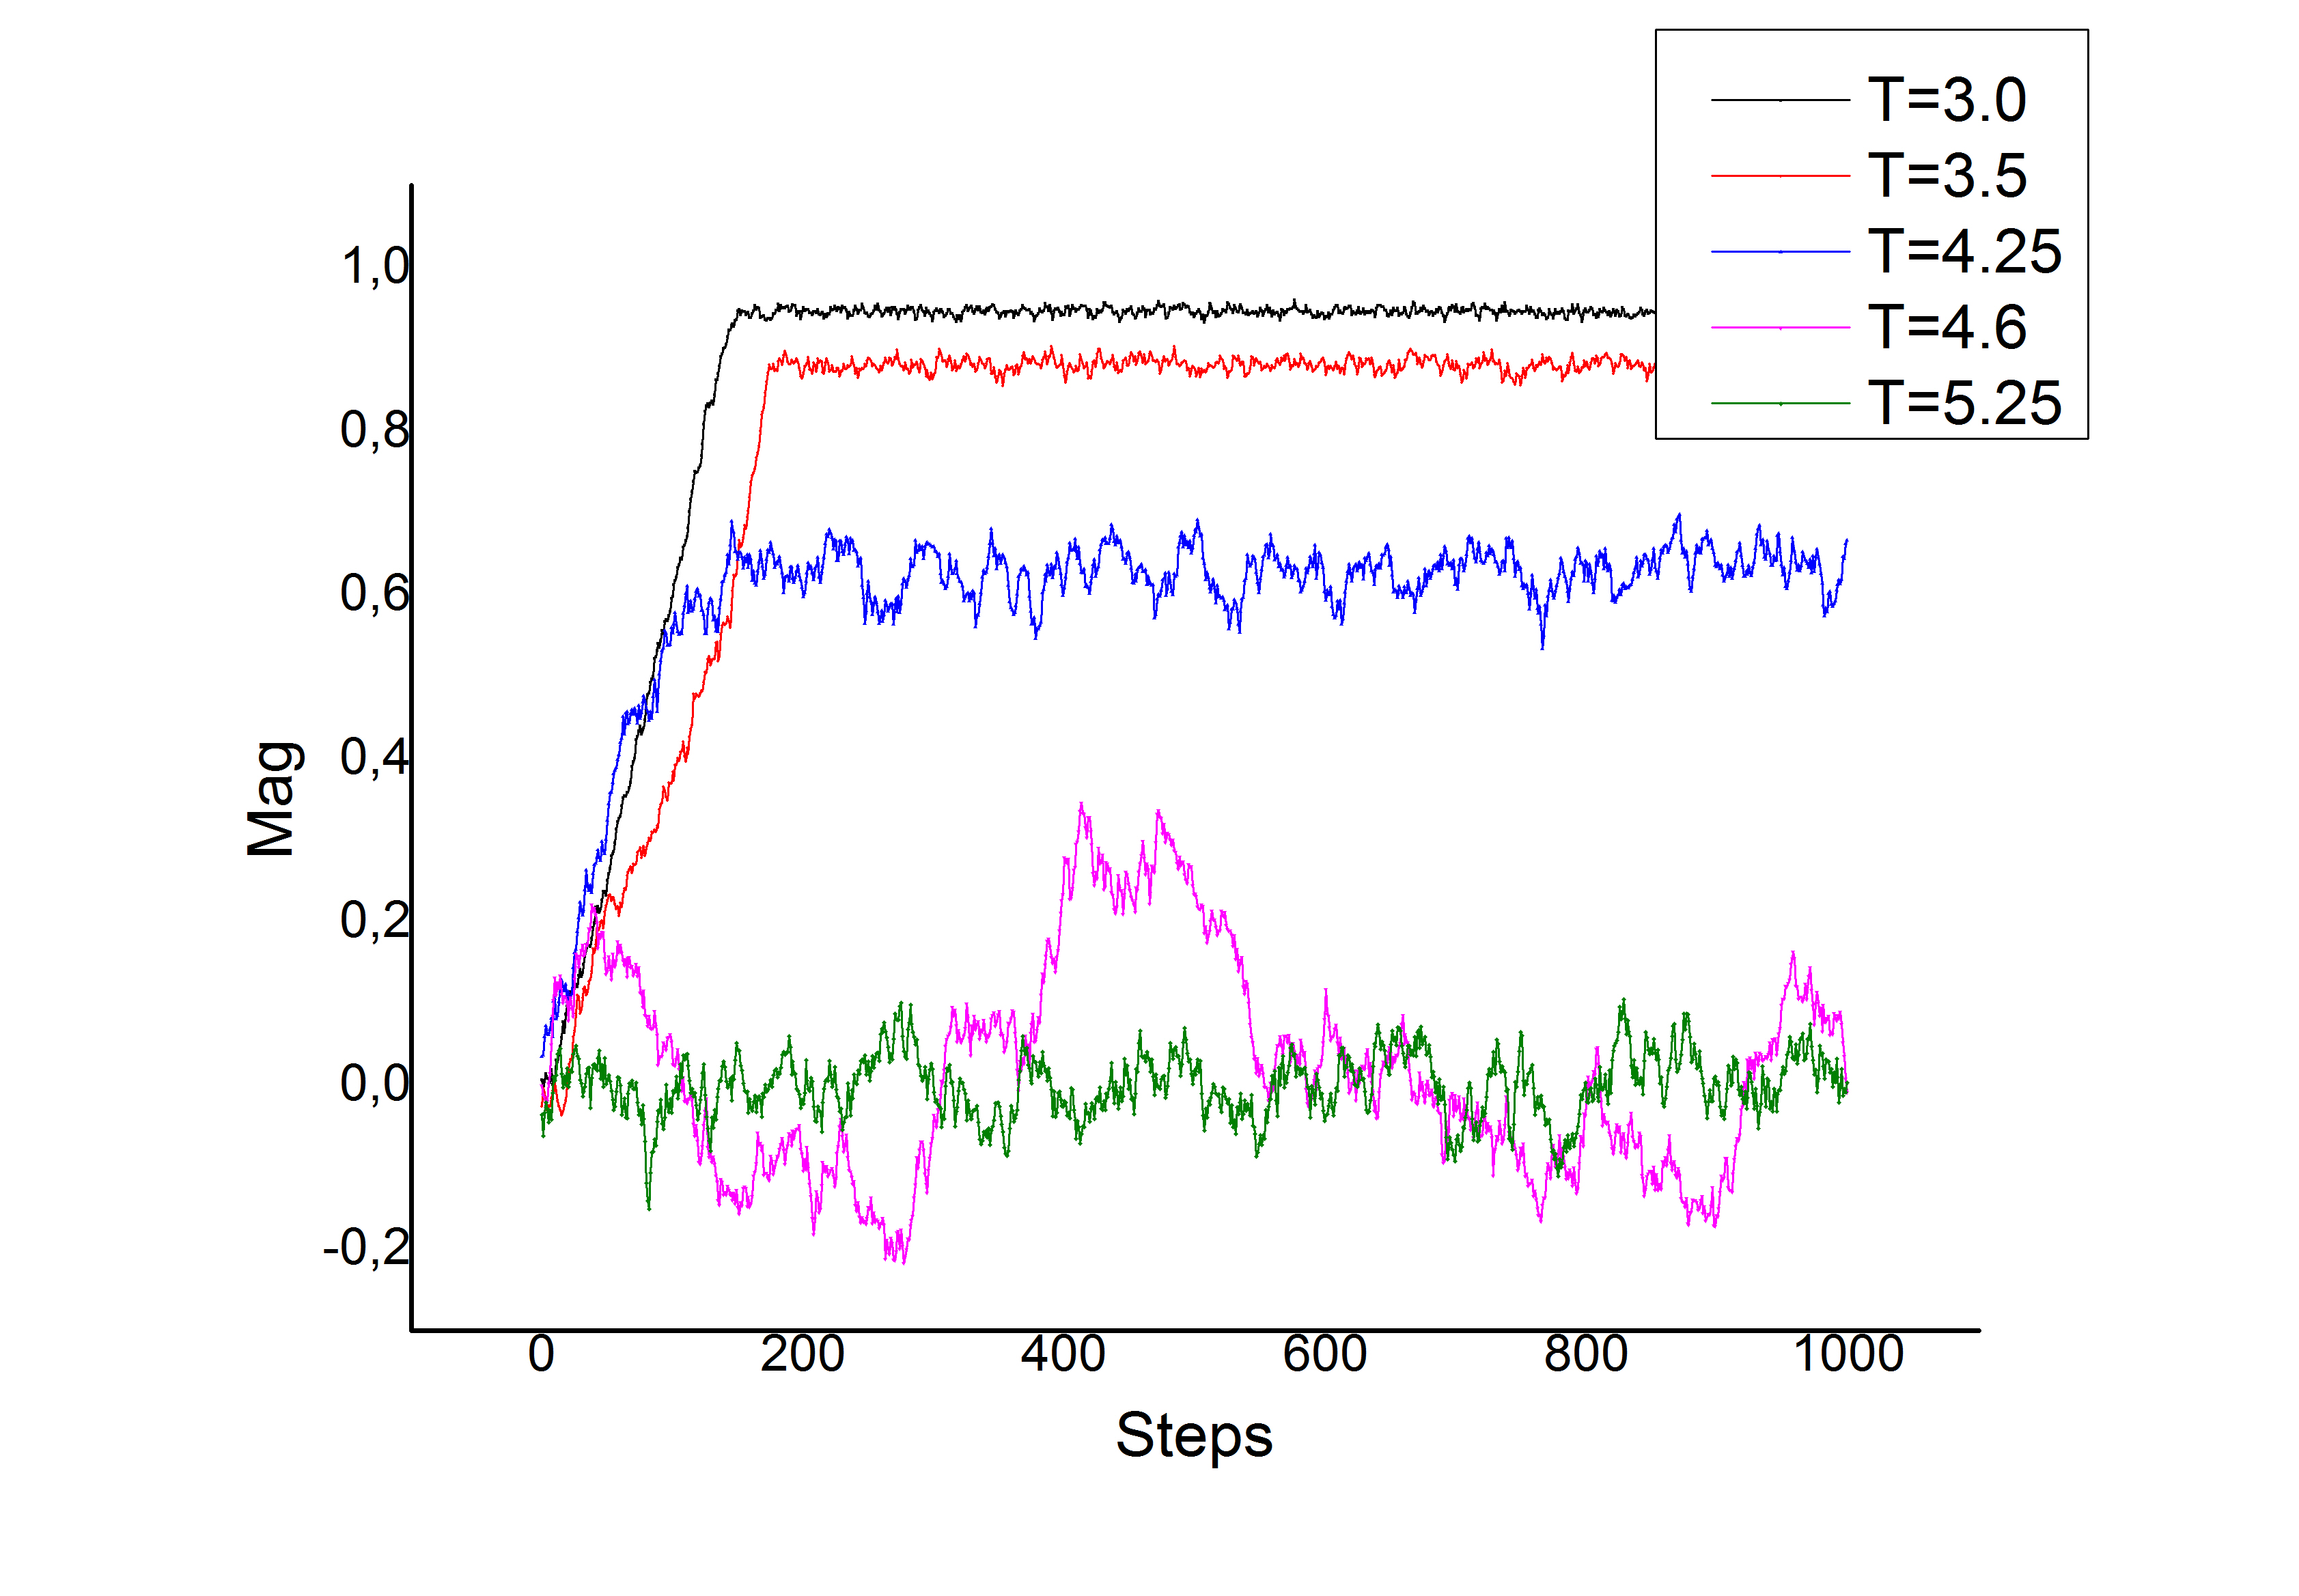
\includegraphics[width=0.47\textwidth]{../Graph_Export/MP3D/m(Steps)_r.jpg}
}	
	\subfigure[positv parallele Startkonfiguration]{
		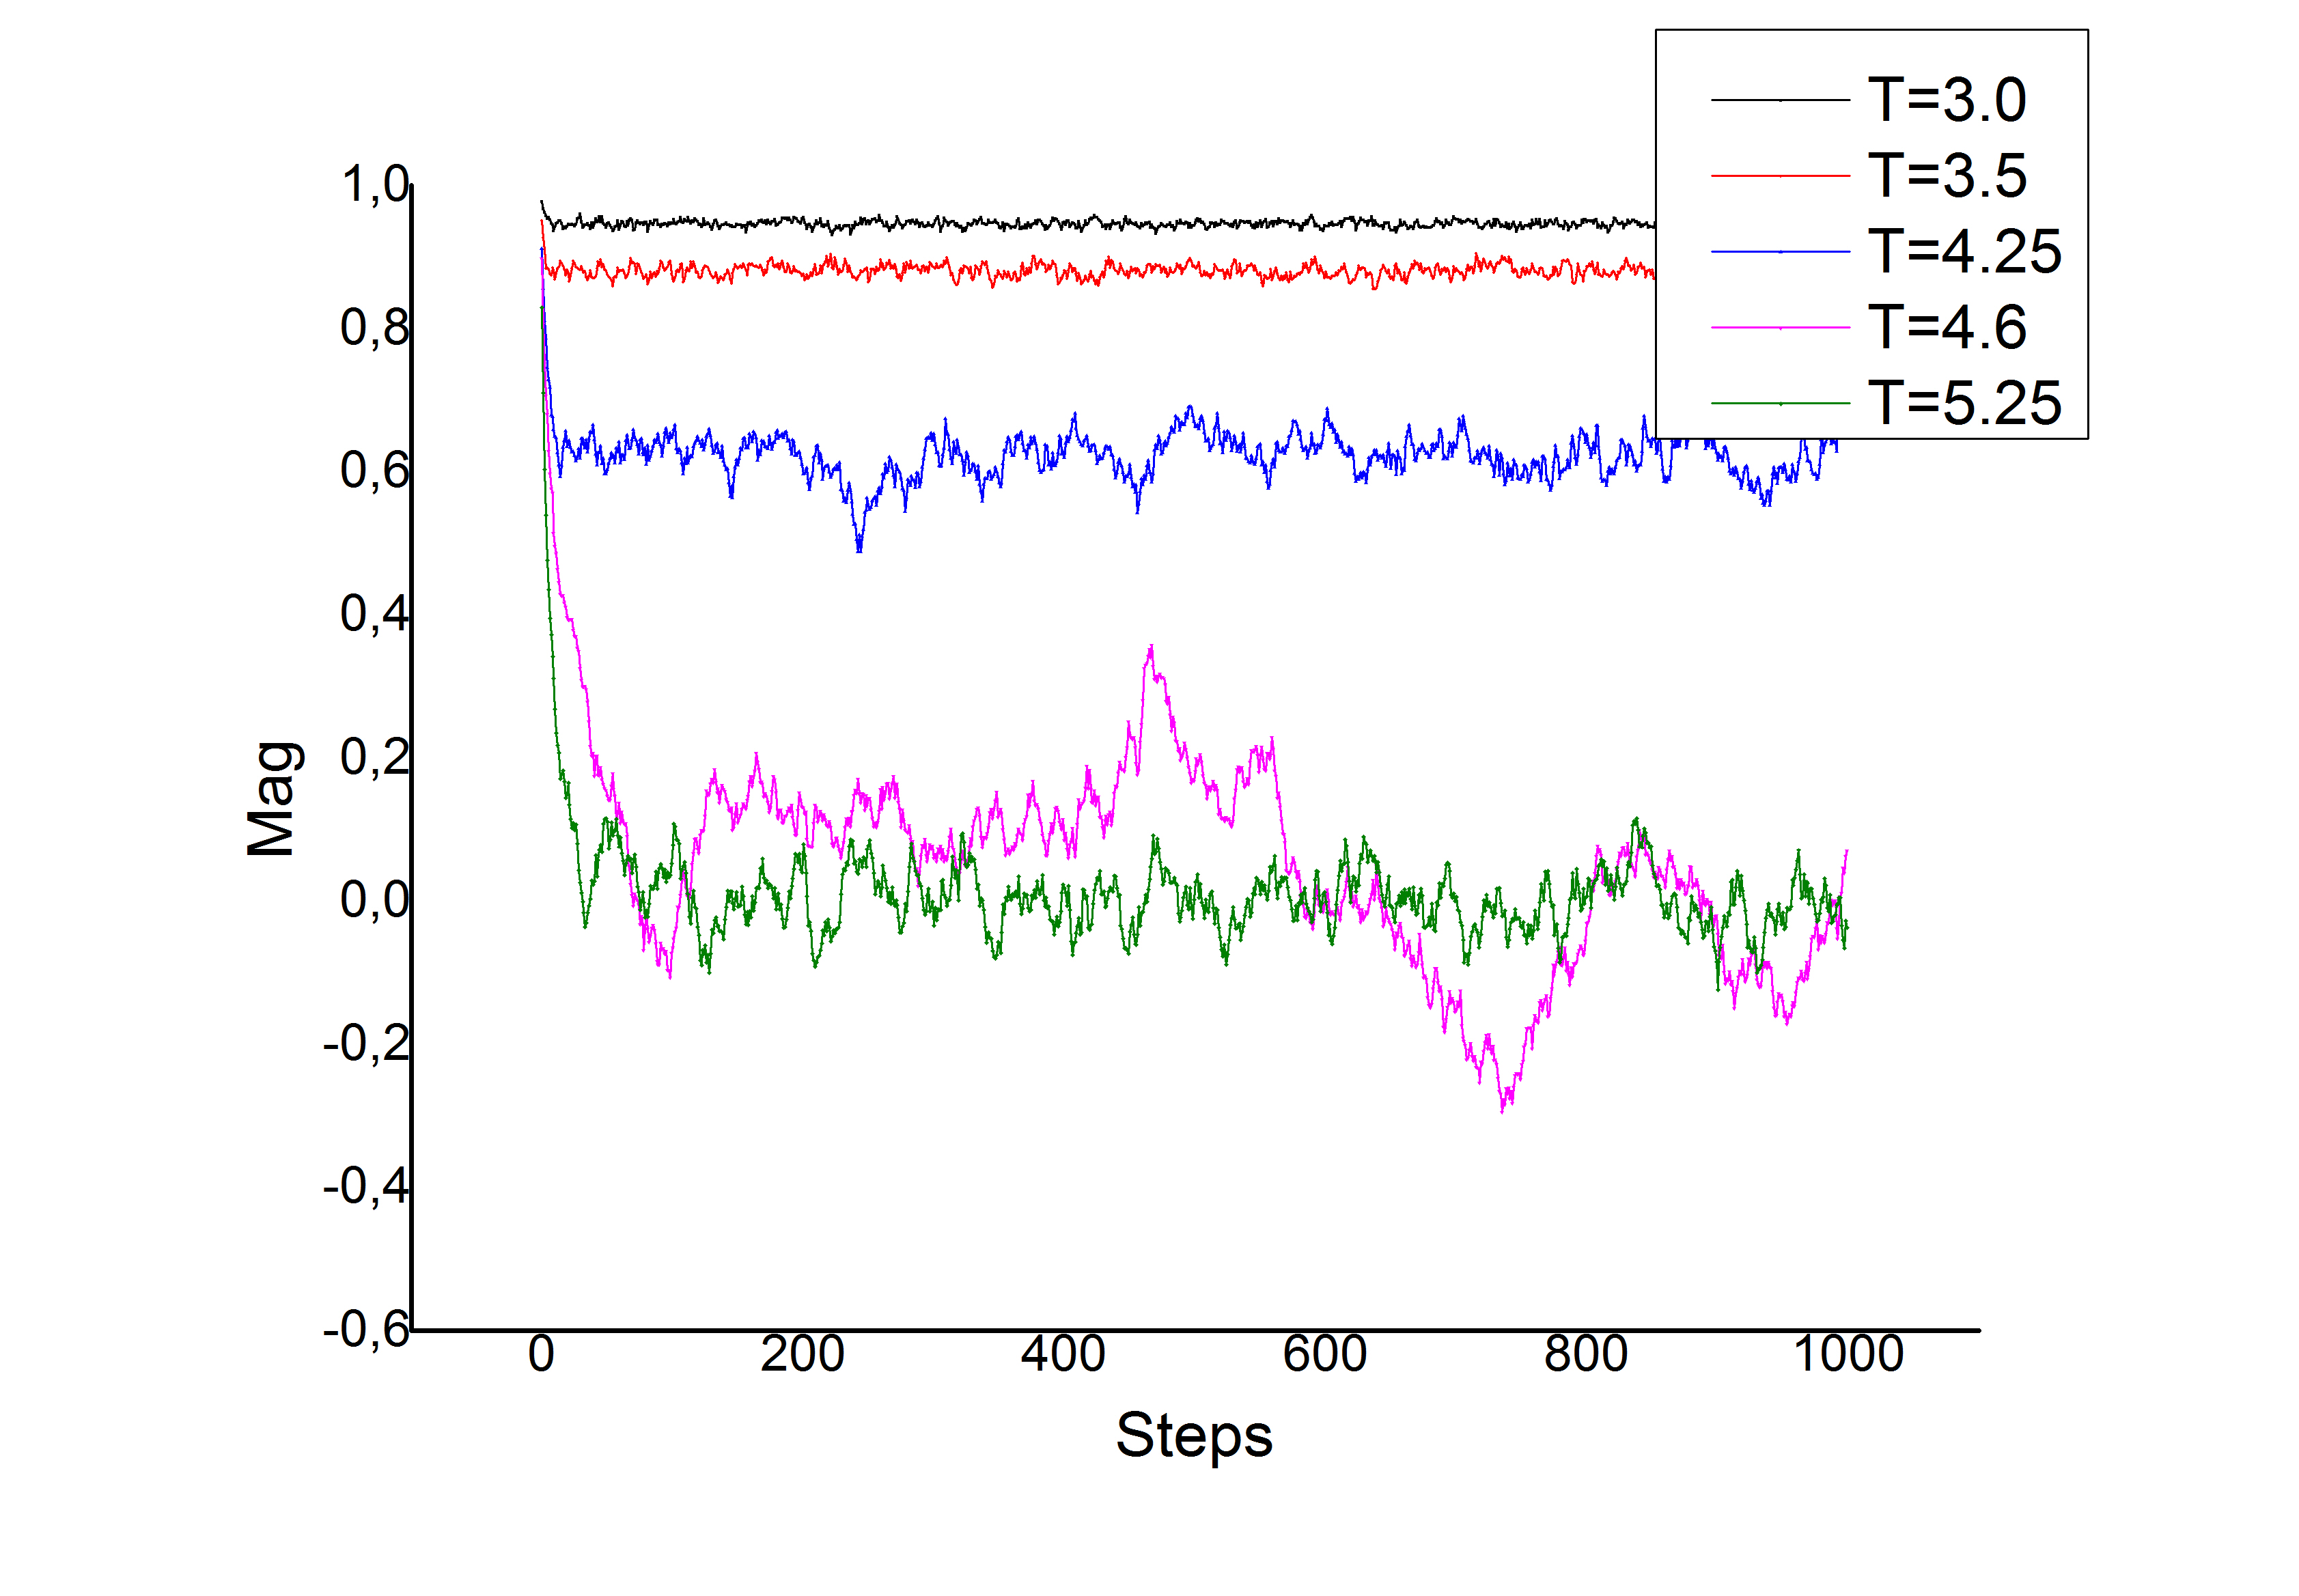
\includegraphics[width=0.47\textwidth]{../Graph_Export/MP3D/m(Steps)_p.jpg}
}		
	\caption{Konvergenzverhalten der Magnetisierung im Metropolisalgorithmus für ein dreidimensionales Gitter}
	\label{mp3dkonv}
\end{figure}

\subsection{Im Detail: Funktion weiterer Parameter}

Unterschied B T Mode etc. ..